\setlength{\footskip}{8mm}

\chapter{METHODOLOGY}

This chapter presents the methodology used to develop AIM-RGL, an agentic MI-CBT framework with reward-guided lookahead search for therapeutic response generation. The chapter describes how the proposed system generates multiple candidate therapist responses, evaluates their possible near-future effects, and selects responses expected to support better therapeutic dialogue outcomes. The methodology is organized around the main AIM-RGL pipeline: multi-agent therapist response generation, reward-guided lookahead search, reward model training, and policy optimization. Client simulation and scenario construction are described as the supporting environment used to generate controlled therapist-client interactions. The study is limited to simulated counseling dialogue and does not aim to diagnose, treat, replace professional therapists, or measure real clinical outcomes.

\begin{figure}[htbp]
    \centering
    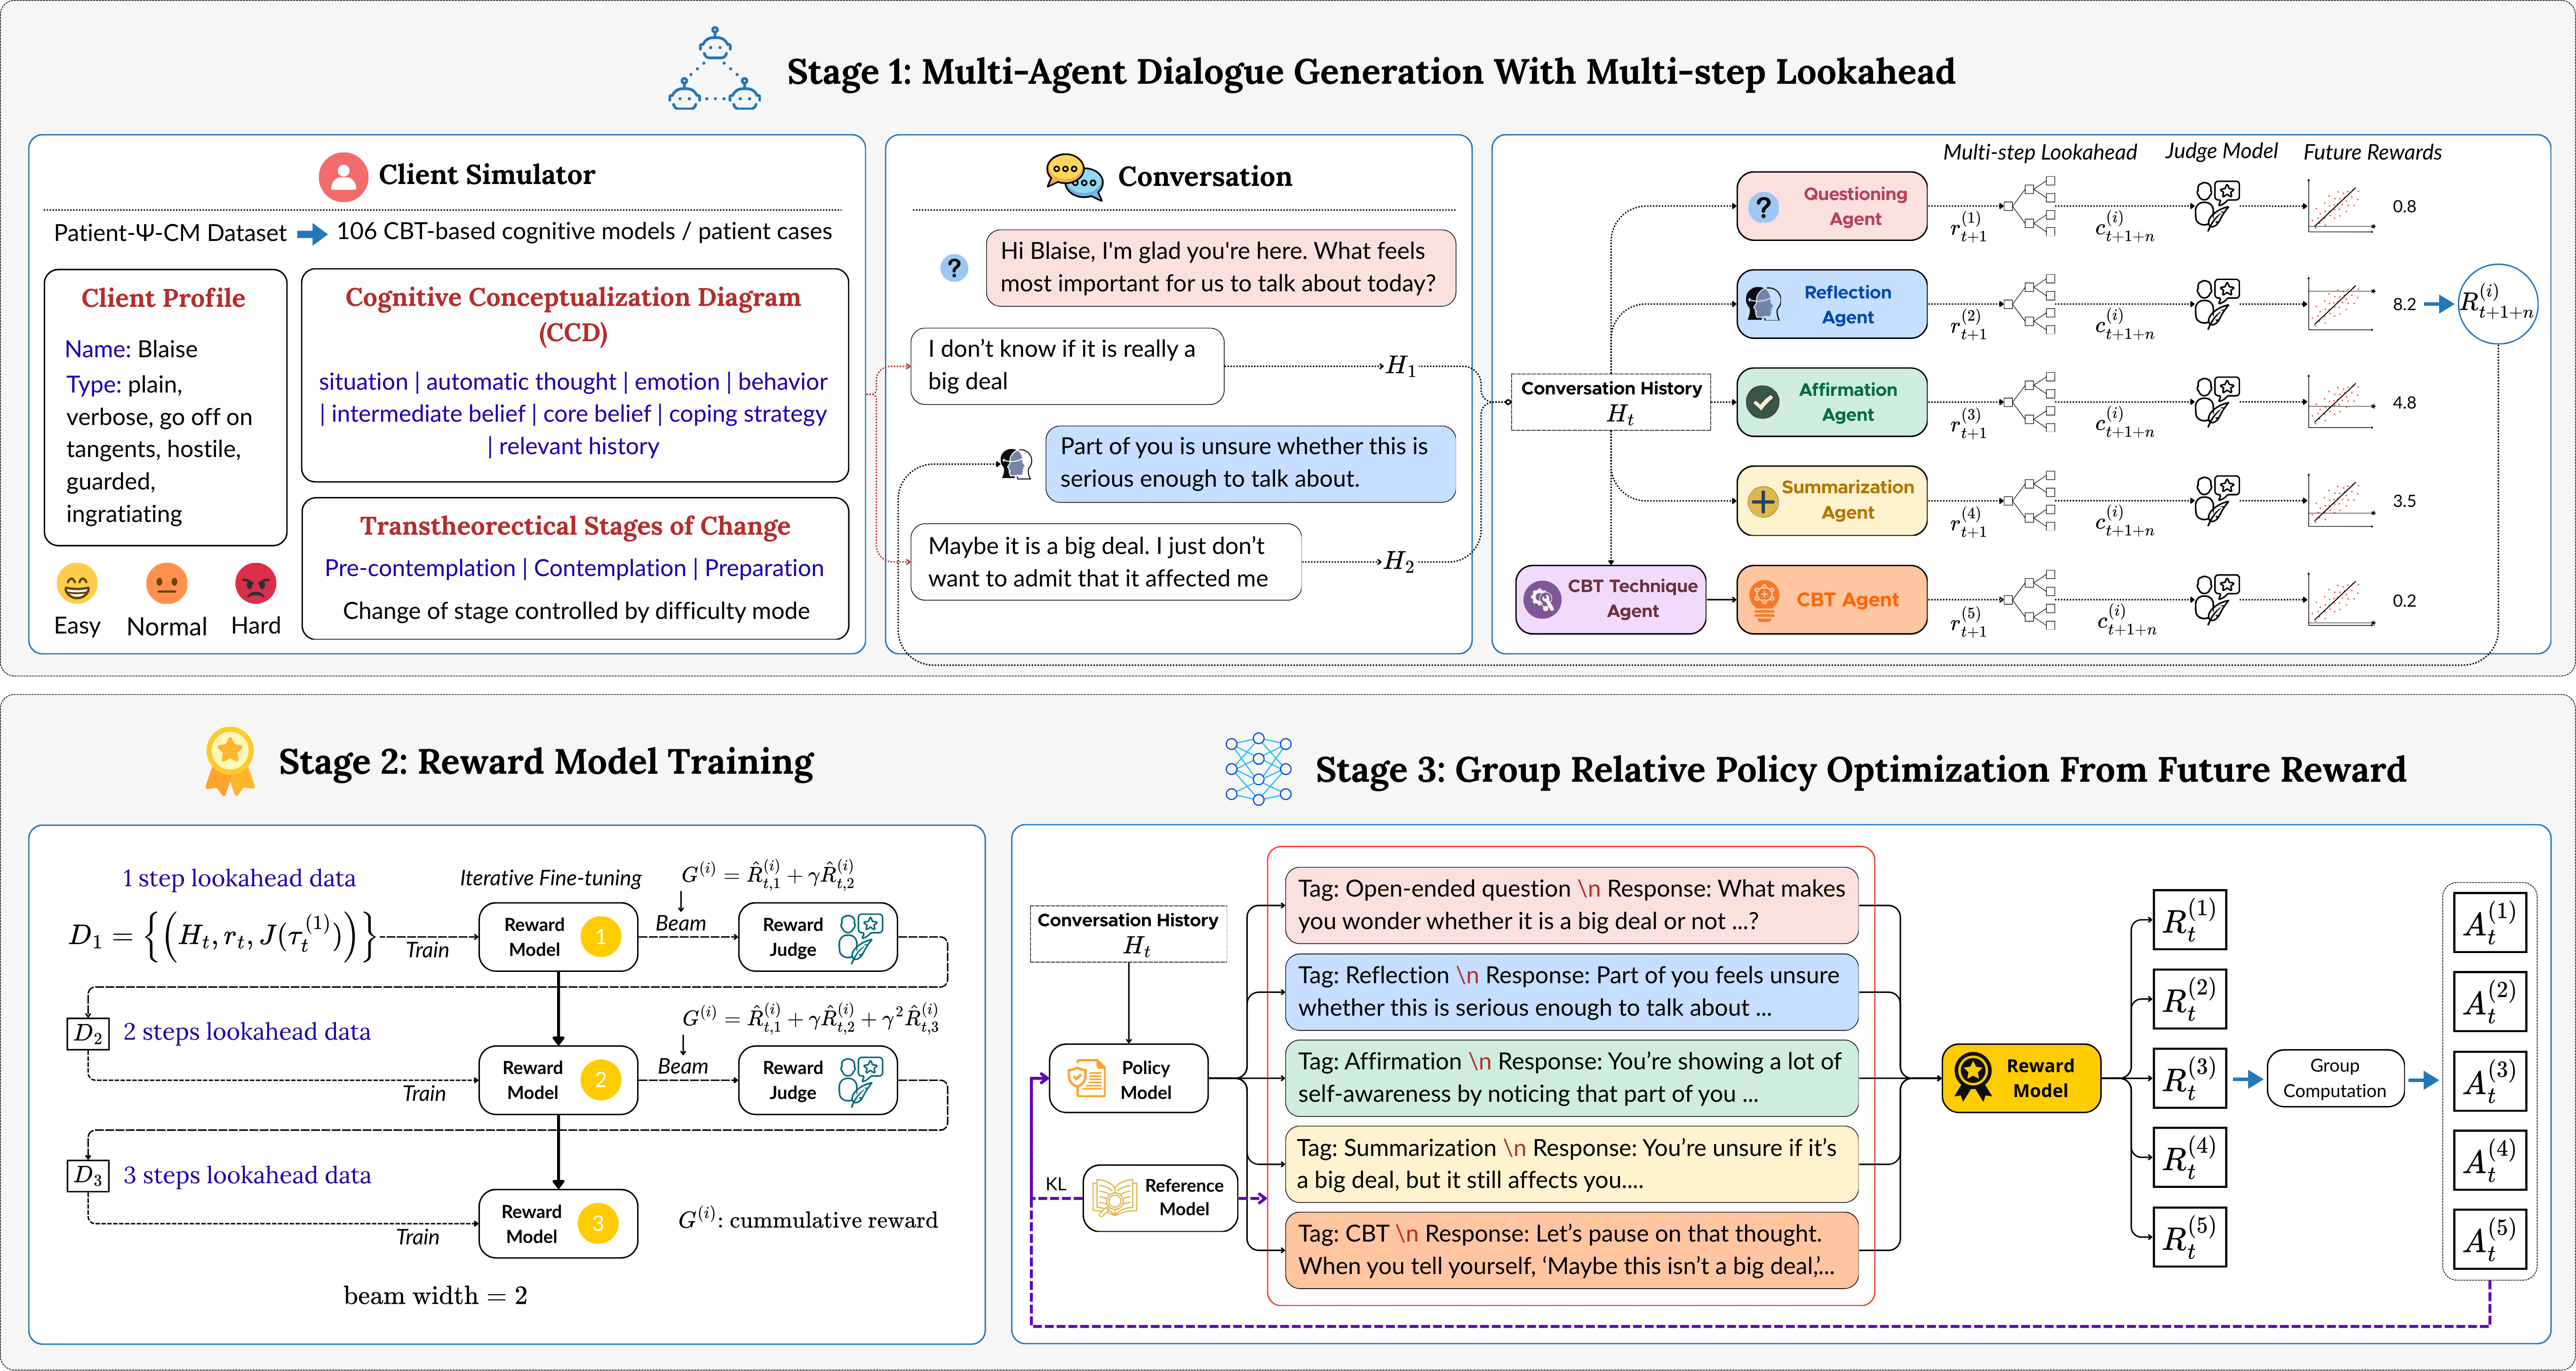
\includegraphics[width=\textwidth]{figures/aim_workflow.png}
    \caption{Overall AIM-RGL workflow, including multi-agent dialogue generation with lookahead, reward model training, and policy optimization from future reward.}
    \label{fig:aim_workflow}
\end{figure}

\section{Research Design and AIM-RGL Framework Overview}

This study adopts a simulation-based system development methodology to design and evaluate AIM-RGL, an agentic MI-CBT framework with reward-guided lookahead search. The main purpose of the methodology is to construct a controlled dialogue framework in which multiple therapeutic responses can be generated, expanded through short-horizon future simulation, evaluated using therapeutic reward signals, and used to guide final response generation. The study focuses on simulated therapist-client dialogue and does not aim to diagnose, treat, replace professional therapists, or measure real clinical treatment outcomes.

AIM-RGL is designed for therapeutic conversations in which the client may show resistance, ambivalence, or changing readiness for structured intervention. In this setting, a response that appears appropriate in the current turn may not necessarily lead to a better next client state. Therefore, the framework treats MI-CBT response generation as a future-aware decision problem. Instead of generating only one therapist response directly, AIM-RGL first generates multiple candidate responses from specialist therapist agents, estimates possible future client reactions, and evaluates the resulting trajectories using therapeutic reward scores.

The overall framework consists of four main components. First, specialist therapist agents generate candidate responses based on different therapeutic skills, including open-ended questioning, reflection, affirmation, summarization, and CBT intervention. Second, reward-guided lookahead search expands these candidates by considering possible near-future dialogue outcomes. Third, a reward model estimates the therapeutic value of candidate responses or trajectories using dimensions such as alliance, empathy, collaboration, CBT skill, MI quality, and client readiness. Fourth, the learned reward signal is used to support policy optimization so that the response generation model can produce therapeutically stronger responses.

The methodology is organized according to this pipeline. Section 3.2 describes the multi-agent therapist response generation process. Section 3.3 explains the reward-guided lookahead search mechanism. Section 3.4 presents reward model training and policy optimization. Section 3.5 describes the simulation environment and client scenario construction used to support the framework. Finally, Section 3.6 discusses the implementation scope and ethical considerations of the study.

\section{Multi-Agent Therapist Response Generation}

AIM-RGL uses a multi-agent therapist architecture to generate candidate responses before the final therapeutic response is selected. The purpose of this stage is not to decide the best response immediately, but to produce a diverse set of therapeutically meaningful options that can later be evaluated through reward-guided lookahead search. Each therapist agent represents a different therapeutic skill or intervention style. This design makes the response generation process more explicit because the framework can compare different MI-style and CBT-style responses instead of relying on a single model to implicitly decide the strategy.

At each therapist turn, the system receives the current conversation history as input. The conversation history includes previous therapist and client utterances, the current client concern, and any available information about the client’s readiness or resistance. Based on this context, the therapist agents generate multiple candidate responses. Each candidate response is tagged with the agent type that produced it, such as open-ended question, reflection, affirmation, summarization, or CBT intervention. These tagged responses form the candidate response pool for the next stage of the framework.

The MI-specific agents are based on the OARS communication skills commonly used in Motivational Interviewing: open-ended questions, affirmations, reflections, and summaries. The open-ended questioning agent generates questions that invite the client to explore thoughts, feelings, goals, and ambivalence in greater depth. The reflection agent mirrors the client’s meaning, emotion, or ambivalence in order to show understanding and reduce defensiveness. The affirmation agent highlights the client’s strengths, effort, values, or persistence in a specific and genuine way. The summarization agent gathers important themes from the conversation and presents them in an organized way to support transition, clarity, or continued exploration.

In addition to MI-specific agents, AIM-RGL includes CBT-specific response generation. The CBT component is divided into two steps. First, a CBT technique selector identifies a suitable CBT technique and plan step for the client’s current concern. Possible techniques include identifying automatic thoughts, evidence-based questioning, alternative perspective taking, decatastrophizing, problem solving, and behavioral experiments. Second, the CBT response agent converts the selected technique and plan step into a brief and natural therapist response. The generated response is written in conversational language and does not need to explicitly name the CBT technique.

The role of the multi-agent stage is to create a balanced response pool that includes both supportive MI-style responses and structured CBT-style responses. This is important because resistant or ambivalent clients may not always be ready for direct cognitive restructuring or action planning. In some cases, a reflective or open-ended MI response may better preserve alliance and reduce resistance. In other cases, when the client shows readiness, a CBT response may help the client examine thoughts or take a concrete step. By generating these alternatives separately, AIM-RGL can later evaluate which response is more likely to support a better near-future therapeutic state.

Table~\ref{tab:therapist_agents} summarizes the main therapist agents used in AIM-RGL.

\begin{table}[htbp]
\centering
\caption{Therapist agents used for candidate response generation.}
\label{tab:therapist_agents}
\begin{tabular}{L{0.25\textwidth}L{0.65\textwidth}}
\toprule
\textbf{Agent} & \textbf{Function} \\
\midrule
Open-ended Questioning Agent & Generates questions that encourage the client to explore thoughts, feelings, goals, and ambivalence. \\
\midrule
Reflection Agent & Reflects the client’s meaning, emotion, or ambivalence to show understanding and reduce defensiveness. \\
\midrule
Affirmation Agent & Highlights the client’s strengths, effort, values, or persistence to support confidence and engagement. \\
\midrule
Summarization Agent & Organizes key themes, emotions, and concerns from the conversation to support clarity and transition. \\
\midrule
CBT Technique Selector & Selects a suitable CBT technique and plan step based on the client’s current concern and readiness. \\
\midrule
CBT Response Agent & Generates a natural therapist response using the selected CBT technique and plan step. \\
\bottomrule
\end{tabular}
\end{table}

The output of this stage is a set of tagged candidate therapist responses. These candidates are not treated as final responses. Instead, they are passed to the reward-guided lookahead search stage, where each response is expanded through simulated future client reactions and evaluated according to its expected therapeutic value.

\section{Reward-Guided Lookahead Search}

After the therapist agents generate candidate responses, AIM-RGL applies reward-guided lookahead search to select the response with the highest expected therapeutic value. The purpose of this stage is to avoid selecting a response only because it appears appropriate in the current turn. Instead, the framework estimates how each candidate response may influence the simulated client’s near-future state, including engagement, resistance, readiness, and therapeutic alliance.

At therapist turn \(t\), the conversation history is denoted as \(H_t\). The multi-agent therapist module generates a set of candidate responses:

\[
A_t = \{r_t^{(1)}, r_t^{(2)}, \ldots, r_t^{(N)}\}
\]

where \(r_t^{(i)}\) is the candidate response generated by therapist agent \(i\), and \(N\) is the number of candidate responses. In this thesis, the main candidate responses are generated by the open-ended questioning, reflection, affirmation, summarization, and CBT agents. Figure~\ref{fig:one_step_lookahead} illustrates this one-step reward-guided lookahead process. Starting from the current conversation history, AIM-RGL generates multiple therapist candidate responses, simulates one possible client response for each candidate, assigns a reward score to each resulting trajectory, and selects the response with the highest reward.

\begin{figure}[htbp]
\centering
\resizebox{\textwidth}{!}{%
\begin{tikzpicture}[
    >=Latex,
    box/.style={
        draw,
        rounded corners=6pt,
        align=center,
        text width=2.25cm,
        minimum height=0.82cm,
        inner xsep=4pt,
        inner ysep=4pt,
        font=\scriptsize
    },
    topbox/.style={
        box,
        fill=blue!12,
        text width=2.60cm,
        font=\scriptsize\bfseries
    },
    clientbox/.style={
        box,
        fill=orange!10,
        text width=2.60cm,
        font=\scriptsize\bfseries
    },
    agentbox/.style={
        box,
        fill=white,
        text width=2.25cm,
        minimum width=2.55cm,
        minimum height=1.15cm,
        text=blue!70!black,
        font=\scriptsize\bfseries
    },
    futurebox/.style={
        box,
        fill=orange!18,
        text width=2.25cm,
        text=brown!70!black
    },
    scorebox/.style={
        box,
        fill=yellow!35,
        text width=2.25cm,
        text=brown!60!black,
        font=\scriptsize\bfseries
    },
    selectedbox/.style={
        box,
        fill=green!10,
        draw=green!45!black,
        text width=4.6cm,
        text=green!35!black,
        font=\scriptsize\bfseries
    },
    arrow/.style={->, thick, shorten >=3pt, shorten <=3pt},
    brace/.style={decorate, decoration={brace, amplitude=6pt, mirror}, thick, draw=gray!75},
    labeltext/.style={font=\scriptsize, align=left}
]

% Top input context
\node[topbox] (history) at (0,0) {Conversation History\\$H_t$};
\node[clientbox] (client) at (0,-1.60) {Current Client\\Utterance};

\draw[arrow] (history.south) -- (client.north);

% Candidate response layer
\node[agentbox] (q)  at (-6.4,-3.80) {Open-ended\\Question};
\node[agentbox] (r)  at (-3.2,-3.80) {Reflection};
\node[agentbox] (a)  at (0,-3.80) {Affirmation};
\node[agentbox] (s)  at (3.2,-3.80) {Summarization};
\node[agentbox] (c)  at (6.4,-3.80) {CBT\\Intervention};

% Branch line from current client utterance to candidates
\coordinate (branch) at (0,-2.70);
\draw[arrow] (client.south) -- (branch);
\draw[thick] (-6.4,-2.70) -- (6.4,-2.70);

\draw[arrow] (-6.4,-2.70) -- (q.north);
\draw[arrow] (-3.2,-2.70) -- (r.north);
\draw[arrow] (0,-2.70) -- (a.north);
\draw[arrow] (3.2,-2.70) -- (s.north);
\draw[arrow] (6.4,-2.70) -- (c.north);

% Simulated future client response layer
\node[futurebox] (cq) at (-6.4,-5.90) {Simulated Client\\Response\\$c_{t+1}^{(1)}$};
\node[futurebox] (cr) at (-3.2,-5.90) {Simulated Client\\Response\\$c_{t+1}^{(2)}$};
\node[futurebox] (ca) at (0,-5.90) {Simulated Client\\Response\\$c_{t+1}^{(3)}$};
\node[futurebox] (cs) at (3.2,-5.90) {Simulated Client\\Response\\$c_{t+1}^{(4)}$};
\node[futurebox] (cc) at (6.4,-5.90) {Simulated Client\\Response\\$c_{t+1}^{(5)}$};

\draw[arrow] (q.south) -- (cq.north);
\draw[arrow] (r.south) -- (cr.north);
\draw[arrow] (a.south) -- (ca.north);
\draw[arrow] (s.south) -- (cs.north);
\draw[arrow] (c.south) -- (cc.north);

% Reward score layer
\node[scorebox] (sq) at (-6.4,-7.85) {Reward\\$R_t^{(1)}$};
\node[scorebox] (sr) at (-3.2,-7.85) {Reward\\$R_t^{(2)}$};
\node[scorebox] (sa) at (0,-7.85) {Reward\\$R_t^{(3)}$};
\node[scorebox] (ss) at (3.2,-7.85) {Reward\\$R_t^{(4)}$};
\node[scorebox] (sc) at (6.4,-7.85) {Reward\\$R_t^{(5)}$};

\draw[arrow] (cq.south) -- (sq.north);
\draw[arrow] (cr.south) -- (sr.north);
\draw[arrow] (ca.south) -- (sa.north);
\draw[arrow] (cs.south) -- (ss.north);
\draw[arrow] (cc.south) -- (sc.north);

% Selection layer
\node[selectedbox] (selected) at (0,-10.10)
{Selected Response\\$r_t^*=\arg\max_i R_t^{(i)}$};

\draw[arrow] (sq.south) -- (-6.4,-9.00);
\draw[arrow] (sr.south) -- (-3.2,-9.00);
\draw[arrow] (sa.south) -- (0,-9.00);
\draw[arrow] (ss.south) -- (3.2,-9.00);
\draw[arrow] (sc.south) -- (6.4,-9.00);
\draw[thick] (-6.4,-9.00) -- (6.4,-9.00);
\draw[arrow] (0,-9.00) -- (selected.north);

% Side braces
\draw[brace] (-7.80,0.50) -- (-7.80,-4.35)
    node[midway, left=8pt, labeltext] {Input};
\draw[brace] (-7.80,-7.35) -- (-7.80,-8.35)
    node[midway, left=8pt, labeltext] {Target};

\node[labeltext, anchor=west] at (7.85,-3.80) {Therapist candidate\\responses};
\node[labeltext, anchor=west] at (7.85,-5.90) {One-step lookahead\\future client responses};
\node[labeltext, anchor=west] at (7.85,-7.85) {Future reward\\scores};

\end{tikzpicture}
}
\caption{One-step reward-guided lookahead search for evaluating therapist candidate responses.}
\label{fig:one_step_lookahead}
\end{figure}

For each candidate response, the client simulator generates a possible future client response. This produces a one-step future trajectory for each candidate:

\[
\tau_t^{(i,1)} = (H_t, r_t^{(i)}, c_{t+1}^{(i)})
\]

where \(c_{t+1}^{(i)}\) is the simulated client response after candidate response \(r_t^{(i)}\). The resulting trajectory is evaluated by a reward judge or reward model:

\[
R_t^{(i)} = J(H_t, r_t^{(i)}, c_{t+1}^{(i)})
\]

where \(J\) represents the reward judge, and \(R_t^{(i)}\) is the reward score assigned to candidate \(i\). The reward score estimates the therapeutic value of the candidate response and its immediate future effect. It is based on therapeutic dimensions such as therapeutic alliance, empathy, collaboration, CBT skill, MI quality, and client readiness.

The selected therapist response is the candidate with the highest estimated reward:

\[
r_t^* = \arg\max_{r_t^{(i)} \in A_t} R_t^{(i)}
\]

This one-step formulation allows AIM-RGL to compare how different MI-CBT responses may affect the client immediately after the therapist turn. For example, a CBT response may appear useful in the current turn, but if the simulated client reacts with stronger resistance or lower readiness, its reward score may be lower than an MI-style reflection or open-ended question.

AIM-RGL also extends this process to multi-step lookahead. Instead of evaluating only the next client response, the framework estimates the cumulative therapeutic value of a response trajectory over a lookahead depth \(d\). The cumulative value of trajectory \(i\) is computed as:

\[
G_t^{(i)} = \sum_{k=1}^{d} \gamma^{k-1}\hat{R}_{t,k}^{(i)}
\]

where \(G_t^{(i)}\) is the cumulative reward of trajectory \(i\), \(d\) is the lookahead depth, \(\gamma\) is the discount factor, and \(\hat{R}_{t,k}^{(i)}\) is the predicted reward at lookahead step \(k\). When \(\gamma = 1\), all future steps are treated equally. When \(\gamma < 1\), earlier rewards are given greater importance than later rewards.

For deeper lookahead, fully expanding all possible branches becomes computationally expensive because each therapist candidate can lead to multiple future client states and additional therapist responses. To reduce this cost, AIM-RGL uses beam-based pruning. After the one-step reward model \(RM_1\) is trained, it is used to estimate the reward of first-step candidate responses. Only the top-ranked candidates are retained as beam branches and expanded further to construct the two-step lookahead dataset \(D_2\). The same procedure is later applied using \(RM_2\) to support three-step lookahead data generation. In this way, the framework avoids expanding the entire search tree while still preserving the most promising therapeutic trajectories for further evaluation.

The final selected response is therefore not simply the response with the best immediate wording. It is the response expected to produce the most beneficial near-future therapeutic trajectory. In the MI-CBT setting, this is important because the system must decide whether the client needs further motivational support, a structured CBT intervention, or a gradual transition between MI and CBT.

\section{Reward Model Training and Policy Optimization}

After candidate trajectories are generated through reward-guided lookahead search, AIM-RGL trains a reward model to estimate the therapeutic value of therapist responses without requiring the reward judge to score every candidate during later stages. The reward model is trained as a regression model that predicts a scalar reward score from the conversation history and a candidate therapist response. This allows the framework to approximate therapeutic reward more efficiently during multi-step lookahead and policy optimization.

Reward model training is carried out through an iterative fine-tuning process across increasing lookahead depths. The reward model is first trained on one-step lookahead data, where each candidate therapist response is evaluated after one simulated client response. After this first-stage reward model is trained, it is used to guide beam-based generation of two-step lookahead data by retaining only the most promising candidate branches. The same process is then repeated for three-step lookahead, allowing the reward model to gradually learn from deeper therapeutic trajectories while reducing the cost of expanding all possible dialogue branches. Figure~\ref{fig:iterative_reward_training} summarizes this iterative reward model training process.

\begin{figure}[htbp]
\centering
\resizebox{\textwidth}{!}{%
\begin{tikzpicture}[
    >=Latex,
    box/.style={
        draw,
        rounded corners=6pt,
        align=center,
        text width=2.45cm,
        minimum width=2.70cm,
        minimum height=1.05cm,
        inner xsep=5pt,
        inner ysep=5pt,
        font=\scriptsize
    },
    datasetbox/.style={
        box,
        fill=blue!6,
        text=blue!70!black,
        font=\scriptsize\bfseries
    },
    rewardbox/.style={
        box,
        fill=white,
        font=\scriptsize\bfseries
    },
    judgebox/.style={
        box,
        fill=yellow!25,
        text=brown!60!black,
        font=\scriptsize\bfseries
    },
    genbox/.style={
        box,
        fill=green!8,
        text=green!35!black,
        font=\scriptsize\bfseries
    },
    mathlabel/.style={
        font=\scriptsize,
        align=center
    },
    arrow/.style={
        ->,
        thick
    },
    feedback/.style={
        ->,
        thick,
        dashed,
        draw=gray!70
    },
    beamlabel/.style={
        font=\scriptsize,
        fill=white,
        inner sep=1pt
    },
    circlelabel/.style={
        circle,
        fill=yellow!80!orange,
        inner sep=2pt,
        minimum size=0.42cm,
        font=\scriptsize\bfseries
    }
]

% Row 1
\node[datasetbox] (d1) at (-5.8,0) {$D_1$\\1-step data};
\node[rewardbox] (rm1) at (-1.7,0) {Reward\\Model};
\node[circlelabel] at (rm1.north east) {1};
\node[judgebox] (judge1) at (2.9,0) {Reward\\Judge};
\node[genbox] (gen2) at (7.1,0) {Generate\\$D_2$};

% Row 2
\node[datasetbox] (d2) at (-5.8,-2.8) {$D_1 \cup D_2$\\2-step data};
\node[rewardbox] (rm2) at (-1.7,-2.8) {Reward\\Model};
\node[circlelabel] at (rm2.north east) {2};
\node[judgebox] (judge2) at (2.9,-2.8) {Reward\\Judge};
\node[genbox] (gen3) at (7.1,-2.8) {Generate\\$D_3$};

% Row 3
\node[datasetbox] (d3) at (-5.8,-5.6) {$D_1 \cup D_2 \cup D_3$\\3-step data};
\node[rewardbox] (rm3) at (-1.7,-5.6) {Reward\\Model};
\node[circlelabel] at (rm3.north east) {3};
\node[mathlabel] (final) at (4.6,-5.6) {Final reward model\\for policy optimization};

% Training arrows
\draw[arrow] (d1.east) -- node[above, font=\scriptsize] {Train} (rm1.west);
\draw[arrow] (d2.east) -- node[above, font=\scriptsize] {Fine-tune} (rm2.west);
\draw[arrow] (d3.east) -- node[above, font=\scriptsize] {Fine-tune} (rm3.west);

% Beam-guided generation arrows
\draw[arrow] (rm1.east) -- node[beamlabel, above=2pt, midway] {Beam search} (judge1.west);
\draw[arrow] (judge1.east) -- node[above, font=\scriptsize] {Score} (gen2.west);
\draw[arrow] (rm2.east) -- node[beamlabel, above=2pt, midway] {Beam search} (judge2.west);
\draw[arrow] (judge2.east) -- node[above, font=\scriptsize] {Score} (gen3.west);
\draw[arrow] (rm3.east) -- (final.west);

% Iterative feedback arrows
\draw[feedback] (gen2.south) -- ++(0,-0.65) -| node[pos=0.25, below, font=\scriptsize] {Add} (d2.north);
\draw[feedback] (gen3.south) -- ++(0,-0.65) -| node[pos=0.25, below, font=\scriptsize] {Add} (d3.north);

% Reward equations
\node[mathlabel] at (5.05,0.95)
{$G^{(i)}=\hat{R}_{t,1}^{(i)}+\gamma\hat{R}_{t,2}^{(i)}$};
\node[mathlabel] at (5.05,-1.85)
{$G^{(i)}=\hat{R}_{t,1}^{(i)}+\gamma\hat{R}_{t,2}^{(i)}+\gamma^2\hat{R}_{t,3}^{(i)}$};

\node[font=\scriptsize\itshape] at (-1.7,0.95) {Iterative fine-tuning};
\node[font=\scriptsize] at (-4.15,-6.55) {beam width \(=2\)};
\node[mathlabel] at (5.0,-6.55) {$G^{(i)}$: cumulative reward};

\end{tikzpicture}
}
\caption{Iterative reward model fine-tuning with beam-guided generation of multi-step lookahead data.}
\label{fig:iterative_reward_training}
\end{figure}

The reward target is first produced by a reward judge. For each candidate trajectory, the reward judge evaluates the response according to multiple therapeutic dimensions, including therapeutic alliance, understanding and empathy, collaboration and structure, CBT skill and strategy, and MI quality and readiness. The overall reward score is computed as the average of these dimension scores:

\[
R = \frac{S_{\text{alliance}} + S_{\text{empathy}} + S_{\text{collaboration}} + S_{\text{CBT}} + S_{\text{MI}}}{5}
\]

where each \(S\) represents the score assigned to one therapeutic dimension. This scalar reward score is used as the training target for the reward model.

Let \(f_{\theta}\) denote the trained reward model with parameters \(\theta\). Given the conversation history \(H_t\) and a candidate therapist response \(r_t^{(i)}\), the reward model predicts:

\[
\hat{R}_t^{(i)} = f_{\theta}(H_t, r_t^{(i)})
\]

where \(\hat{R}_t^{(i)}\) is the predicted therapeutic reward for candidate response \(i\). The model is trained to minimize the difference between the predicted reward \(\hat{R}_t^{(i)}\) and the reward target \(R_t^{(i)}\) assigned by the reward judge. The training objective is formulated using mean squared error:

\[
\mathcal{L}_{RM} = \frac{1}{M}\sum_{m=1}^{M}\left(\hat{R}_m - R_m\right)^2
\]

where \(M\) is the number of training samples, \(\hat{R}_m\) is the reward predicted by the reward model, and \(R_m\) is the reward target assigned by the reward judge.

Reward model training is performed iteratively across different lookahead depths. In the one-step stage, the system constructs the dataset \(D_1\) by generating candidate therapist responses, simulating one future client response for each candidate, and assigning reward scores to the resulting one-step trajectories. The first reward model \(RM_1\) is trained using this one-step lookahead dataset:

\[
RM_1 = Train(M_0, D_1)
\]

where \(M_0\) is the pretrained base model used as the initial reward model backbone.

After \(RM_1\) is trained, it is used to support two-step lookahead data generation. Instead of expanding all candidate branches, \(RM_1\) scores the first-step candidate responses and retains only the top-ranked candidates as beam branches. These retained branches are then expanded further to generate two-step trajectories. The resulting dataset is denoted as \(D_2\). The second reward model \(RM_2\) is then fine-tuned using both one-step and two-step lookahead data:

\[
D_2 = Generate(RM_1, d=2)
\]

\[
RM_2 = FineTune(RM_1, D_1 \cup D_2)
\]

The same procedure is repeated for three-step lookahead. The trained \(RM_2\) is used to guide branch selection and generate the three-step lookahead dataset \(D_3\). The third reward model \(RM_3\) is then fine-tuned using all available lookahead datasets:

\[
D_3 = Generate(RM_2, d=3)
\]

\[
RM_3 = FineTune(RM_2, D_1 \cup D_2 \cup D_3)
\]

This iterative training process allows the reward model to gradually learn from deeper future trajectories while reducing the computational cost of exhaustive search. The beam-based procedure keeps the most promising branches for expansion, making multi-step lookahead more practical.

After reward model training, the learned reward signal is used to optimize the therapist response policy. For each conversation history \(H_t\), the policy model samples a group of candidate therapist responses:

\[
r_t^{(1)}, r_t^{(2)}, \ldots, r_t^{(G)} \sim \pi_{\phi}(\cdot \mid H_t)
\]

where \(\pi_{\phi}\) is the policy model and \(G\) is the number of sampled responses in the group. Each sampled response is scored by the trained reward model:

\[
R_i = RM(H_t, r_t^{(i)})
\]

The rewards are then normalized within the group to compute a relative advantage for each candidate response:

\[
A_i = \frac{R_i - \mu_R}{\sigma_R + \epsilon}
\]

where \(\mu_R\) and \(\sigma_R\) are the mean and standard deviation of the reward scores within the group, and \(\epsilon\) is a small constant used for numerical stability. Responses with higher relative reward receive positive advantages, while lower-scoring responses receive lower or negative advantages.

\subsection{GRPO}

After the reward model is trained, it is used to guide policy optimization. For each conversation history, the policy model samples a group of candidate therapist responses. The trained reward model scores each response, and the scores are normalized within the group to compute relative advantages. These advantages are then used to update the policy model while a KL penalty constrains the updated policy from drifting too far from the reference model. Figure~\ref{fig:grpo_policy_optimization} illustrates this GRPO-based policy optimization process.

\begin{figure}[htbp]
\centering
\resizebox{\textwidth}{!}{%
\begin{tikzpicture}[
    >=Latex,
    box/.style={
        draw,
        rounded corners=6pt,
        align=center,
        text width=2.75cm,
        minimum width=3.05cm,
        minimum height=1.05cm,
        inner xsep=5pt,
        inner ysep=5pt,
        font=\scriptsize
    },
    mainbox/.style={
        box,
        fill=blue!8,
        font=\scriptsize\bfseries
    },
    samplebox/.style={
        box,
        fill=orange!10,
        text width=3.35cm,
        minimum width=3.70cm
    },
    rewardbox/.style={
        box,
        fill=yellow!25,
        font=\scriptsize\bfseries
    },
    advbox/.style={
        box,
        fill=green!10,
        text width=3.10cm,
        minimum width=3.45cm,
        font=\scriptsize\bfseries
    },
    updatebox/.style={
        box,
        fill=purple!8,
        text width=3.10cm,
        minimum width=3.45cm,
        font=\scriptsize\bfseries
    },
    refbox/.style={
        box,
        fill=gray!10,
        font=\scriptsize\bfseries
    },
    arrow/.style={->, thick},
    arrowlabel/.style={font=\scriptsize, fill=white, inner sep=1pt}
]

% Main flow
\node[mainbox] (history) at (-6.0,0) {Conversation History\\$H_t$};

\node[mainbox] (policy) at (-2.6,0) {Policy Model\\$\pi_{\phi}$};

\node[samplebox] (samples) at (1.2,0) {
Sampled Candidate Responses\\
$r_t^{(1)}, r_t^{(2)}, \ldots, r_t^{(G)}$
};

\node[rewardbox] (reward) at (5.4,0) {
Reward Model\\
$R_i = RM(H_t,r_t^{(i)})$
};

\node[advbox] (advantage) at (5.4,-2.45) {
Group-Normalized Advantage\\
$A_i = \dfrac{R_i-\mu_R}{\sigma_R+\epsilon}$
};

\node[updatebox] (grpo) at (1.2,-2.45) {
GRPO Policy Update\\
maximize high-reward responses
};

\node[mainbox] (updated) at (-2.6,-2.45) {
Updated Policy Model\\
$\pi_{\phi}^{new}$
};

% Reference model for KL
\node[refbox] (ref) at (1.2,-4.55) {
Reference Model\\
$\pi_{\text{ref}}$
};

% Arrows
\draw[arrow] (history) -- (policy);
\draw[arrow] (policy) -- (samples);
\draw[arrow] (samples) -- (reward);
\draw[arrow] (reward) -- (advantage);
\draw[arrow] (advantage) -- (grpo);
\draw[arrow] (grpo) -- (updated);

% KL arrow
\draw[arrow, dashed] (ref.north) -- node[arrowlabel, right=2pt] {KL penalty} (grpo.south);

% Feedback arrow
\draw[arrow, dashed] (updated.north) -- node[arrowlabel, right=2pt] {next iteration} (policy.south);

\end{tikzpicture}
}
\caption{GRPO-based policy optimization using rewards predicted by the trained reward model.}
\label{fig:grpo_policy_optimization}
\end{figure}

The policy model is optimized using a group-relative objective. The purpose is to increase the likelihood of responses with higher predicted therapeutic reward while constraining the updated policy from drifting too far from the reference model. This is represented as:

\[
\mathcal{L}_{GRPO}(\phi)
=
-\frac{1}{G}\sum_{i=1}^{G}
\min
\left(
\rho_i A_i,
\text{clip}(\rho_i, 1-\epsilon, 1+\epsilon)A_i
\right)
+
\beta D_{KL}(\pi_{\phi} \| \pi_{\text{ref}})
\]

where

\[
\rho_i = \frac{\pi_{\phi}(r_t^{(i)} \mid H_t)}
{\pi_{\text{old}}(r_t^{(i)} \mid H_t)}
\]

\(\rho_i\) is the probability ratio between the updated policy and the old policy, \(A_i\) is the group-normalized advantage, \(\beta\) controls the strength of the KL penalty, and \(\pi_{\text{ref}}\) is the reference policy model.

Through this process, AIM-RGL uses the trained reward model not only for response selection, but also for improving the response generation policy. The policy optimization stage encourages the model to generate therapist responses that are more likely to support therapeutic alliance, empathy, collaboration, MI-CBT fidelity, and client readiness in simulated dialogue.
